
Рентгеновское излучение, взаимодействуя с электронами атомов вещества, рассеивается.
Ядра атомов в рассеянии рентгеновских лучей практически не участвуют, т.к.
амплитуда электромагнитной волны, рассеянной заряженной частицей, в соответсвии с формулой
Томсона \cite{iveronova1972}, обратно пропорциональна ее массе. Величина рассеяния
на атоме зависит от количества электронов в нем. Тяжелые металлы,
 например свинец (Z = 82), рассеивают рентгеновское излучение сильнее легких,
 таких как никель (Z = 28) или  кобальт (Z = 27), а такие атомы, как гелий или водород, прозрачны
 для рентгеновского излучения.  Атомный множитель $f$ (атомный фактор рассеяния) определяется,
как отношение амплитуды волны, рассеянной одним атомом, к амплитуде волны, рассеянной
одним свободным электроном.

На рис. \ref{ris:atom_factor} в качестве примера представлена диаграмма направленности атомного
фактора лантана в зависимости от угла. Размеры атома соизмеримы с длиной волны
рентгеновских лучей, поэтому между волнами рассеянными отдельными электронами, возникает
разность фаз. Это разность фаз равна нулю только при $2 \theta = 0$, поэтому структурный
фактор зависит от $\theta$ и $\lambda$. Максимальная величина, которая равна числу электронов в атоме $Z$,
 наблюдается в случае рассеяния вперед. Действительно, если в атоме сосредоточено
 $Z$ электронов, то заряд этой группы равен $Q = Z\cdot e$, а масса $M = Z \cdot m_e$.

\begin{figure}[H]
  \centering
  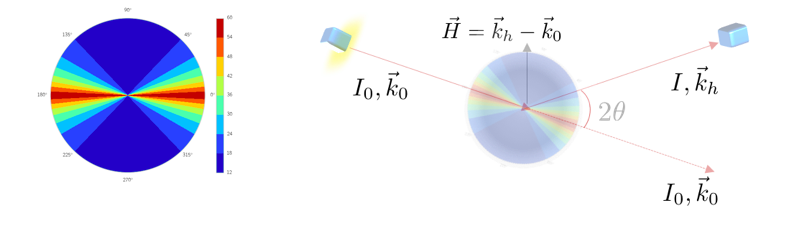
\includegraphics[width=0.9\textwidth]{images/atom_factor.png}
  \caption{Фактор рассеяния для атома лантана (Z = 57) (слева),
  схема расположения векторов для падающей и рассеянной волн (справа)}
  \label{ris:atom_factor}
\end{figure}

Приближенное выражение для расчета атомного фактора рассеяния
представляется в следующем виде \cite{International_Tables}:

\begin{equation}
  f_0 = \sum_{i=1}^{4} \cdot a_i e^{ -b_i (\frac{sin \vartheta_B}{\lambda})^2} + C,
 \end{equation}
где $a_i$, $b_i$ и $c$ - коэффициенты Кромер-Манна для бездисперсионного канала рассеяния атомами решетки.
Характерная зависимость структурного фактора от угла рассеяния и длины волны
для атомов входящих, например, в состав кристалла LGT (La, Ga, Ta, O), являющегося
одним из объектов исследования в настоящей работе, представлена на рис. \ref{ris:atom_factor_GaLaTa}.

\begin{figure}[H]
  \centering
  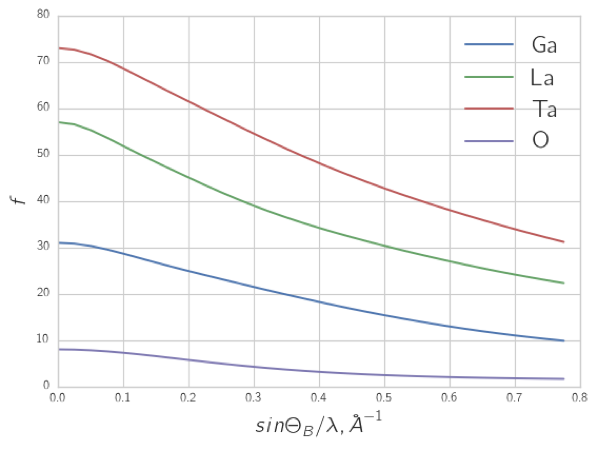
\includegraphics[width=0.6\textwidth]{images/atom_factor_GaLaTa.png}
  \caption{ Атомный фактор рассеяния для атомов: галлия (Ga), лантана (La), тантала (Ta) и  кислорода (O)}
  \label{ris:atom_factor_GaLaTa}
\end{figure}

При расчете интенсивности рассеяния атомом необходимо учитывать,
что все электроны связаны между собой. Для этого необходимо рассматривать
уравнение движение связанного электрона под действием падающего излучения.
Если атом многоэлектронный, то амплитуда рассеянной волны равна сумме амплитуд волн,
рассеянных всеми электронами атома, в результате структурный фактор $f$
определяется выражением \cite{iveronova1972}:

\begin{equation}
  f = f_0 + f^{'} + i f^{''},
 \end{equation}
\noindent
где $f_0$ - атомный фактор рассеяния, рассчитанный без учета сил связи электронов
 с ядром, а $f^{'}$ и $f^{''}$ - дисперсионные поправки \cite{f0f1f12},
 первая из которых учитывает дополнительное рассеяние,
а вторая - дополнительное поглощение вблизи собственных частот колебаний электронов в атоме.

 \begin{figure}[H]
   \centering
   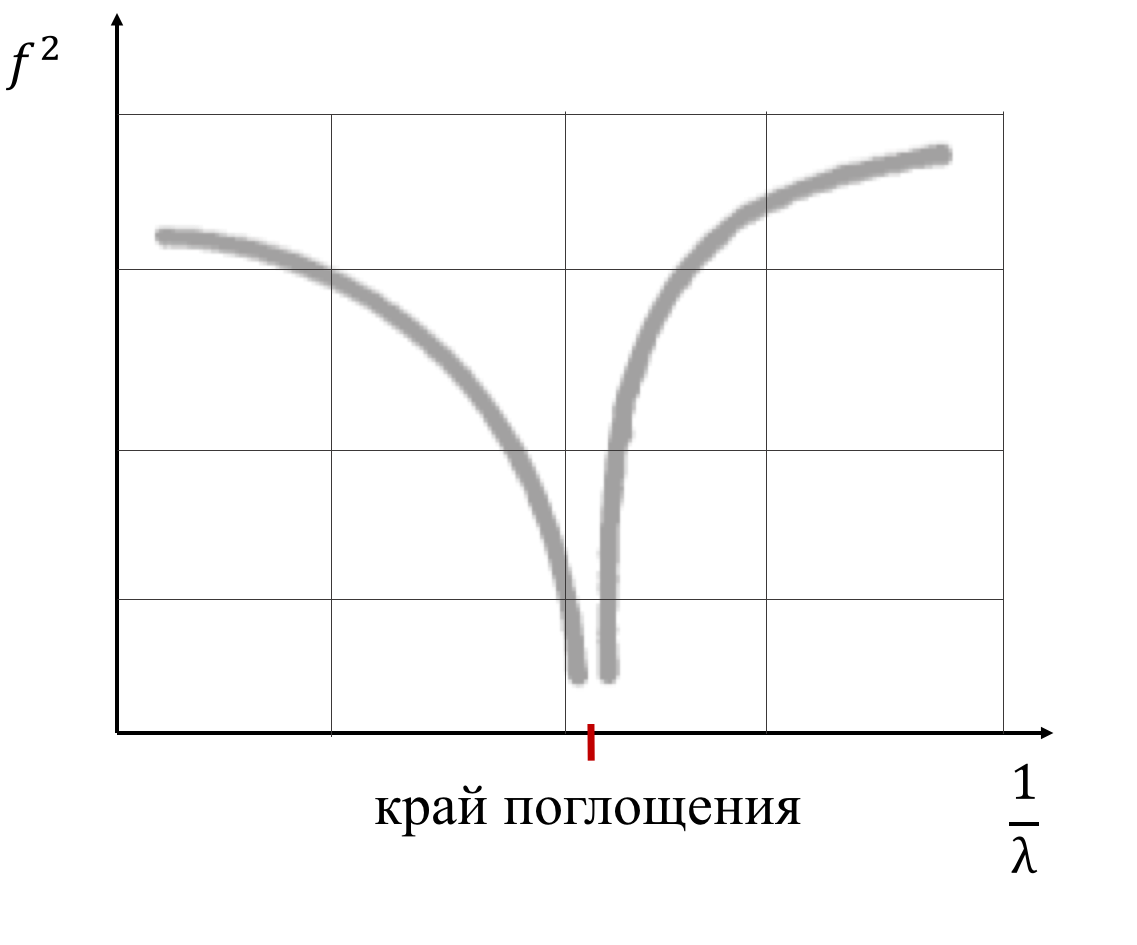
\includegraphics[width=0.4\textwidth]{images/dispers_f.png}
   \caption{ Схематичная зависимость квадрата атомного фактора $f^2 = (f_0 + f^{'})^2 + (f^{''})^2 $ от
   длины волны $\lambda$ вблизи края поглощения}
   \label{ris:dispers_f}
\end{figure}

Важной особенностью является тот факт, что дисперсионные поправки $f^{'}$, $f^{''}$
практически не зависят от угла рассеяния, но зависят от энергии. Так как $f_0$ уменьшается
с ростом угла рассеяния, при больших углах $\theta$ все большую роль начинают играть дисперсионные поправки.
